\documentclass[letterpaper]{article}
\usepackage[]{float}
\usepackage[utf8]{inputenc}
\usepackage[T1]{fontenc}
\usepackage{textcomp}
\usepackage[dutch]{babel}
\usepackage{amsmath, amssymb}
\usepackage[margin=1.3in]{geometry}
\usepackage{import}
\usepackage{xifthen}
\pdfminorversion=7
\usepackage{pdfpages}
\usepackage{transparent}
\newcommand{\incfig}[1]{%
	\def\svgwidth{\columnwidth}
	\import{./figures/}{#1.pdf_tex}
}
\usepackage[]{fancyhdr}
\pdfsuppresswarningpagegroup=1

\setlength\parindent{0pt}
\begin{document}
\pagestyle{fancy}
\fancyhead{} % clear all header fields
\fancyhead[L]{PHYS301 : Classical Mechanics}
\fancyhead[C]{\rightmark}
\fancyhead[R]{Homework 05}
\fancyfoot{}
\renewcommand{\footrulewidth}{0.4pt}

\newlength\adder
\setlength\adder{1cm}
\addtolength\headwidth{2\adder}
\fancyheadoffset{\adder}

\fancyfoot[C]{\vspace{0.3cm}\\ \thepage}


\begin{center}
\ 
	\vspace{1cm} 

	\Huge{\textsf{Homework 05 : : Classical Mechanics}}
	\\
	\vspace{1cm}
	\Large{\texttt{Ahmed Saad Sabit}}
	\vspace{1.5cm} 
\end{center}
{\flushright
\section*{Answer Sheet} 
}
\vspace{0.3cm}
\textbf{Problem 01} 

\noindent\rule{\textwidth}{0.2pt} 
\begin{itemize}
	\item Fourier representation: 
		\[ f(x) = \frac{2}{ \pi } + \sum_{n=1}^{\infty} \left(\frac{4}{\pi (1- 4n^2 )}\right) \cos(2 n x) \] 
	\item Plots of the Representation: Plotted in solution. 
\end{itemize}


\vspace{0.4cm}
\textbf{Problem 02}\\
\noindent\rule{\textwidth}{0.2pt} 
\begin{itemize}
	\item Work by impulse case \[W = \frac{K^2}{2m}\]  Work by Damped Spring Computation: \[
			W = \frac{K^2}{\sqrt{\omega_0^2 - \gamma^2} } \qquad \text{or, with mass } \frac{K^2}{m \sqrt{\omega_0^2 - \gamma^2} }
	\] 
\item Mistake of statement: (summary) impulse given by force is non-zero hence particle does achieve some speed hence $v(0)=0$ cannot be assumed.  
\end{itemize}

\vspace{0.4cm}
\textbf{Problem 03} \\
\noindent\rule{\textwidth}{0.2pt} 
\begin{itemize} 
	\item Response solution \[
 x(t) = F_0 \sum_{n=0}^{\infty} A^{n} G\left(t, \frac{n}{2} \tau\right)  
=  F_0 \sum_{n=0}^{\infty} 
A^{n}
\Theta(t - n \tau / 2 ) 
\frac{e^{- \gamma (t- n \tau / 2)}}{\omega}  
\sin\left[\omega (t- n \tau / 2 )\right]
\] 
\item The amplitude of oscillation can be written as $\Lambda^{n} e^{- \gamma t} \frac{1}{\omega}$ where $\Lambda = A e^{\gamma \tau / 2}$ setting the bound 
	\[
	e^{- \gamma \tau / 2} > A 
	\] 
\item Exponential Increase. 
\end{itemize}
\newpage
\ 

{\center{\section*{\textsf{Problem 01}} }}
\vspace{0.7cm} 

First of all note that $y(x) = | \sin(x) | $ is an even function as
\[
f(-x) = f(x)
\] This function representation is a periodic function where $\tau = \pi$
\[
y(x) = \sin(x) \quad (0 \le x \le \pi = \tau)
\]
The function repeats itself after every $x = \tau$. Basic common sense. 
For this our Fourier Series representation of this problem would be with period $\tau = \frac{2\pi}{\omega } = \pi$ as $\omega = 2$
\[
f(x) = a_0 + \sum_{n=1}^{\infty} a_n \cos(\omega n x) 
\]

\textbf{Solve for $a_0$: } 

\begin{align*} 
	\int_{0}^{\tau}  
	f(x) \, \mathrm{d} x &= \int_{0}^{\tau}   a_0 \mathrm{d} x + \int_{0}^{\tau}  \sum_{n=1}^{\infty} a_n \cos(\omega n x) \, \mathrm{d} x \\ 
	&\implies
a_0 = \frac{1}{\tau} \int_{0}^{\tau} f(x) \, \mathrm{d} x 
	\\
\end{align*}

\textbf{Solve for $a_n$:}
\begin{align*}
	\int_{0}^{\tau} f(x) \cos(\omega p x) &= 
\int_{0}^{\tau}  a_0 \cos(\omega p x) \, \mathrm{d}  x + \sum_{n=1}^{\infty} 
\int_{0}^{\tau} a_n  \cos(\omega n x) \cos(\omega p x) \, \mathrm{d}  x
	\\  
\int_{0}^{\tau} f(x) \cos( \omega p x) &=
a_p \frac{\pi}{\omega} \tag{2nd term is zero for $n \neq p$} 
\\ 
a_p &= \frac{\omega}{\pi } \int_{0}^{\tau} f(x) \cos(\omega p x)   \, \mathrm{d} x\\
\end{align*}
\textbf{Putting together:} 
\[
f(x) = \frac{1}{\pi} \int_{0}^{\tau} f(x) \, \mathrm{d} x + 
\frac{2}{\pi } \int_{0}^{\tau} f(x) \cos(2 px)  \, \mathrm{d} x
\]
\textbf{Computation of $a_0$: }
\begin{align*} a_0 &= \frac{1}{ \pi }
	\int_{0}^{\tau} \sin(x) \, \mathrm{d} x = \frac{2}{\pi }
\end{align*}

\textbf{Computation of $a_p$ : }
\begin{align*} a_p &=  \frac{2}{\pi }
	\int_{0}^{\tau} \sin(x) \cos(2 p x) \, \mathrm{d}  x   \\
	&= \frac{2}{\pi } \frac{2}{1 - 4p^2} \\
	&= \frac{4}{\pi (1 - 4 p^2)} \\
\end{align*}
Hence the series repsentation is 
\[
\boxed{
f(x) = \frac{2}{ \pi } + \sum_{n=1}^{\infty} \left(\frac{4}{\pi (1- 4n^2 )}\right) \cos(2 n x)
}
\] 
\textbf{Visual Analysis: }
\begin{figure}[H]
	\centering
	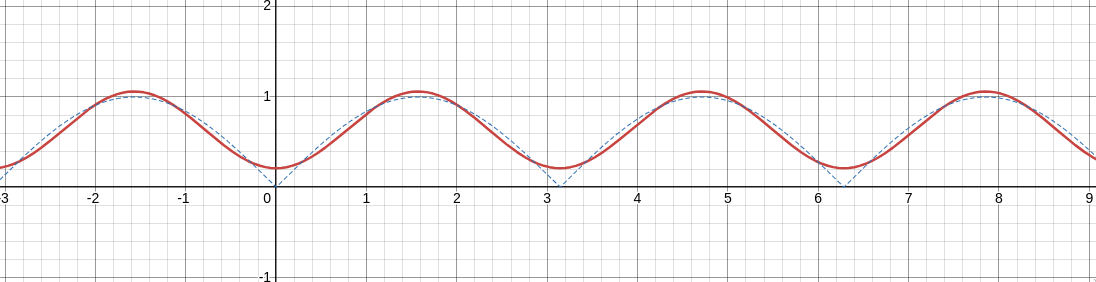
\includegraphics[width=0.8\textwidth]{ss/5/p1-1.png}
	\caption{$n = 1$ for summation, dotted line for actual $| \sin(x) |$ plot.}
	\label{fig:ss-5-p1-1-png}
\end{figure}
\begin{figure}[H]
	\centering
	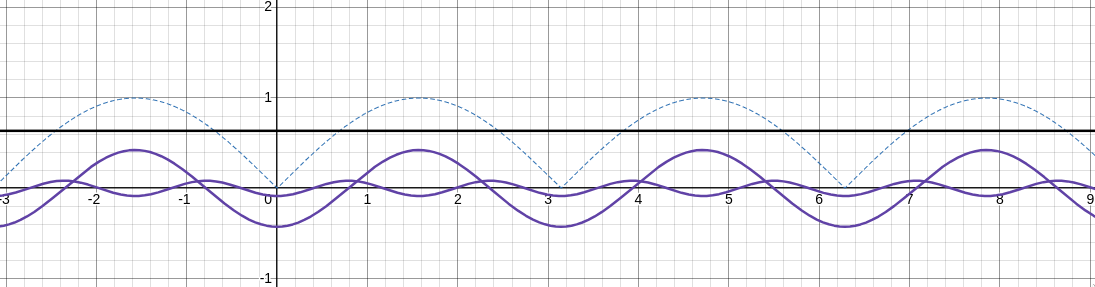
\includegraphics[width=0.8\textwidth]{ss/5/p1-2.png}
	\caption{First three terms of the series are plotted.}
	\label{fig:ss-5-p1-1-png}
\end{figure}
\begin{figure}[H]
	\centering
	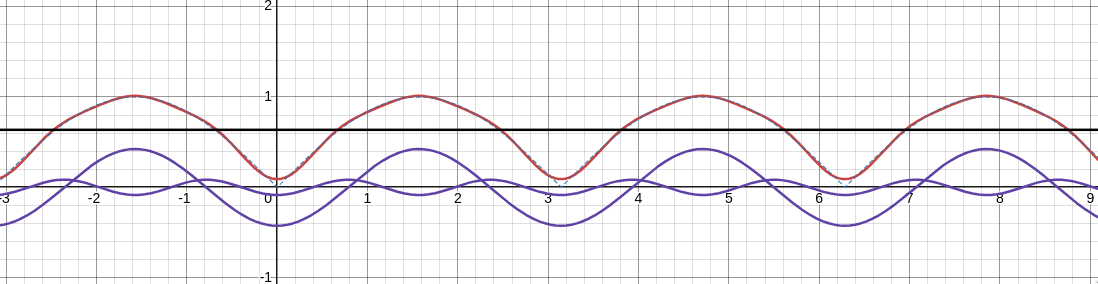
\includegraphics[width=0.8\textwidth]{ss/5/p1-3.png}
	\caption{Red plot shows the summation of the three lines (can be compared with blue dotted exact plot).}
	\label{fig:ss-5-p1-1-png}
\end{figure}


\newpage
{\center{\section*{\textsf{Problem 02}}}
}
\textbf{Impulsive force on free particle:}
\[
\int F(t) \, \mathrm{d} t =  \int K \delta(t) \, \mathrm{d} t = K = \Delta P = m v - 0 = mv \implies
v = \frac{K}{m}
\]
\textbf{NOTE:} As instructed in office hours, if we consider the particle to behave like a free particle, then work done here is $W = (1 / 2) m v^2 - 0 = K^2 / 2 m $ 
\[
W = \frac{K^2}{2 m}
\] 
\vspace{0.2cm}
\textbf{Damped Spring System:} To keep things simple consider $m=1$
\[
\ddot{x} + 2 \gamma \dot{x} + \omega_0^2 x = F(t) = K \delta(t)
\]
We had defined Green's Function for this specific use case 
\[
	\left( \frac{\mathrm{d} ^2}{\mathrm{d} t^2} + 
		2 \gamma \frac{\mathrm{d} }{\mathrm{d} t} + 
		\omega_0^2
	\right) x(t) =
	\left( \frac{\mathrm{d} ^2}{\mathrm{d} t^2} + 
		2 \gamma \frac{\mathrm{d} }{\mathrm{d} t} + 
		\omega_0^2
	\right) G(t,0) \cdot K = K \delta(t)
\] 
\begin{align*}  x(t) = 
 K G(t,0) = \frac{\Theta(t)}{\omega} \sin\left(\omega t\right) e^{- \gamma t} \qquad (\omega ^2 = \omega_0^2 - \gamma^2 )
\end{align*}  

\begin{align*}
 v(0) = \frac{\mathrm{d} x(t)}{\mathrm{d} t} \Biggr\vert_{t = 0 } &= \lim_{\epsilon \to 0} \frac{x(\epsilon)	- 
	x(0 ) }{ \epsilon}  \\ &= 
\lim_{\epsilon \to 0}  \frac{1}{\epsilon} 
\left(
	\frac{K}{\omega} \sin(\omega \epsilon) e^{- \gamma \epsilon} 
\right) \\
&\approx
\frac{K}{\omega}
\\
\end{align*}
\textbf{Work done by the impulsive force: }
\begin{align*}
	W = \int_{-\infty}^{\infty} F(t) \left(\frac{\mathrm{d} x}{\mathrm{d} t}\right) \, \mathrm{d} t  &= \int_{-\infty}^{\infty} F(t) v(t) \, \mathrm{d} t  \\ 
	&= \int_{-\infty}^{\infty} K \delta(t) v(t) \, \mathrm{d} t  \\
	&= K \int_{-\infty}^{\infty} v(t) \delta(t) \, \mathrm{d} t  \\
	&= K v(0)  \\
\end{align*}
Note that we cannot make the statement $v(0) = 0$ as the impulsive force has already imparted a momentum on this spring system, hence $|v(0)| > 0$. 

\[
W = K v(0) = K \frac{K}{\omega} = \frac{K^2}{\sqrt{\omega_0^2 - \gamma^2} }
\] 
If we have to consider mass, it's trivial (inspired from Natural Units)
\[
W = \frac{K^2}{m \sqrt{\omega_0^2 - \gamma^2} }
\] 


\newpage{
\center\textsf{\section*{Problem 03} }}
\[
\ddot{x} + 2 \gamma \dot{x} + \omega_0^2 x = F_0 \sum_{n=0}^{\infty} A^{n} \delta \left(t - \frac{n}{2} t\right)
\] 
We know that for the simple case
\[
\ddot{x} + 2 \gamma \dot{x} + \omega_0^2 x = \delta(t -t') \implies x(t) = 
G(t,t')
\] 
We can manipulate this to take the form as given by the force
\begin{align*}
\ddot{x} + 2 \gamma \dot{x} + \omega_0^2 x = \delta\left(t - \frac{n}{2} \tau \right) 
 & \implies x(t) = G\left(t, \frac{n}{2} \tau\right)  \\ 
\ddot{x} + 2 \gamma \dot{x} + \omega_0^2 x = A^{n}\delta\left(t - \frac{n}{2} \tau \right) 
 & \implies x(t) = A^{n} G\left(t, \frac{n}{2} \tau\right)  \\
\ddot{x} + 2 \gamma \dot{x} + \omega_0^2 x =F_0 \sum_{n=0}^{\infty}  A^{n}\delta\left(t - \frac{n}{2} \tau \right) 
 & \implies x(t) = F_0 \sum_{n=0}^{\infty} A^{n} G\left(t, \frac{n}{2} \tau\right)  \\
\end{align*}
Defining  $\omega = \sqrt{\omega_0^2 - \gamma^2 } $

\begin{minipage}{0.4 \textwidth}
\begin{figure}[H]
	\centering
	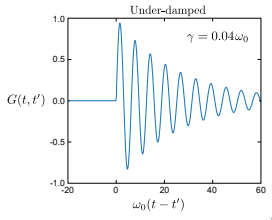
\includegraphics[width=0.9 \textwidth]{ss/5/p3-1.png}
	\label{fig:ss-5-p3-1-png}
\end{figure}  
\end{minipage}\hfill %
\begin{minipage}{0.6\textwidth}
\[
G(t,t') = \Theta(t - t') 
\frac{e^{- \gamma (t-t')}}{\omega}  
\sin\left(\omega (t-t')\right)
\\ \]
\end{minipage}

\vspace{0.3cm}
Hence the response is given by 
\[
x(t) = 
F_0 \sum_{n=0}^{\infty} 
A^{n}
\Theta(t - n \tau / 2 ) 
\frac{e^{- \gamma (t- n \tau / 2)}}{\omega}  
\sin\left[\omega (t- n \tau / 2 )\right]
\]
Or if you, dear grader, would like a concise form 
\[
 x(t) = F_0 \sum_{n=0}^{\infty} A^{n} G\left(t, \frac{n}{2} \tau\right)  
\] 

Let's look at the peaks now. They are given by at any $n \tau / 2 < t < (n+1) \tau / 2	$ 
\[
A^{n} e^{- \gamma ( t - n \tau / 2) } \cdot  \frac{1}{ \omega} = 
A^{n} \left(
e^{ - \gamma t} e^{n \gamma \frac{\tau}{2}} \right) \frac{1}{\omega} = 
\left(A e^{ \gamma \tau /2 }\right) ^{n} e^{-\gamma t} \frac{1}{\omega} = 
\Lambda^{n} e^{- \gamma t} \frac{1}{\omega}
\]
We require $\Lambda < 1$ otherwise $\Lambda^{n}$ will blow up over time. The exponent term $e^{- \gamma t}$ ensures we have a decay.  
\[
A e^{ \gamma \tau / 2} < 1 \implies A < {e^{  - \gamma \tau / 2}}
\] 
Now coming to the fight between $\text{Jay}$ and Kay, we can write the amplitude as $e^{- \gamma \tau / 2} < A < 1$. This obviously causes the terms to increase in magnitude every interval of $ \tau / 2$. Hence it is true that there will be an exponential explosion of amplitude. 
\newpage
\section*{appendix: trashcan}

\begin{align*}
v(0) = 	\dot{x}(t) &= \frac{1}{ \omega K} \left( \frac{\mathrm{d} \Theta(t)}{\mathrm{d} t}\right) + \frac{\Theta(t)}{\omega K}  
\ \frac{\mathrm{d} }{\mathrm{d} t} \left(
\sin\left(\omega t\right) e^{- \gamma t}
\right) \\ 
		   &= 
\frac{\delta(t)}{ \omega K} + \frac{\Theta(t)}{ K} \cos(\omega t) e^{- \gamma t} + \frac{\Theta(t)}{ \omega K} \sin(\omega t) (- \gamma)e^{ - \gamma t}
\end{align*} 

\end{document}
